\providecommand{\main}{../main}
\documentclass[\main/main.tex]{subfiles}
\graphicspath{{../images/}}
\begin{document}
\section{
    くりこみ群
}
\subsection{
    連続極限の気持ち
}\label{subsec: continuum limit}
身の回りにあるマクロな多体系において、単位体積(例えば$\SI{1}{cm^3}$)に含まれている原子の数は$10^{23}$程度の巨大な数である。
場の理論の基本的な思想は、非常に多数の自由度の理想化として、無限の自由度を持つ系を考えることである。
\begin{align}
    10^{23} ≈ ∞
\end{align}
簡単な例として、以下の作用で表される1次元の調和振動子系を考えてみる。
\begin{align}
    S = ∫\dd{t}\Q[\f{1}{2}m ∑_n\.ϕ_n^2 -\f{1}{2}κ∑_n(ϕ_{n+1}-ϕ_n)²]
\end{align}
\begin{figure}[H]
    \centering
    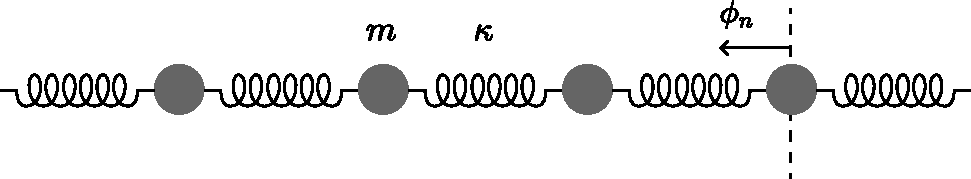
\includegraphics[width=0.7\hsize]{../images/oscillators.pdf}
    \caption{調和振動子系}
\end{figure}
運動方程式を書くと
\begin{align}
    m\dv[2]{t}ϕ_n = κ(ϕ_{n+1}+ϕ_{n-1}-2ϕ_n)
\end{align}
である。
解の形として$ϕ_n = \e^{-\iωt}\e^{\i kan}$を仮定すると、
以下の分散関係を得る。
\begin{align}
    -mω² = κ(\e^{\i ka}+\e^{-\i ka}-2),
    \␣
    ω = \√{\f{2κ}{m}(1-\cos(ka))}
    \label{dispertion relation}
\end{align}
$ka ≪ 1$のときは
\begin{align}
    ω ≈ \√{\f{κa²}{m}}|k| ≕ v|k|
    \label{linear dispertion relation}
\end{align}
という線形な分散関係が得られる。
ここで、$κ,m,a$といった微視的なモデルのパラメーターは全て音速$v$という一つのパラメーターにまとめられていることに注意する。
% (\ref{dispertion relation})は微視的なモデルの詳細による式だが、(\ref{linear dispertion relation})は格子振動において普遍的な式にである。

次に、巨視的な物理量を保つような連続極限を考える。
具体的には密度$ρ = m/a$と張力$T = κa$を保ちながら$a → 0$とする。
このとき$ϕ_n(t) = \√a ϕ(an, t)$として、作用は
\begin{align}
    S = ∫\dd{t}\dd{x}\Q(\f{1}{2}ρ(∂_tϕ)²-\f{1}{2}T(∂_xϕ)²)
    \label{action of string}
\end{align}
となる。また運動方程式は
\begin{align}
    \∂[2]{ϕ}{t} = v²\∂[2]{ϕ}{x},\␣ v = \√{\f{T}{ρ}}
\end{align}
となる。
この理論は古典的ではあるが、場の理論の利点を反映している。
連続化した理論は非加算無限個の自由度を含み、もとの理論よりもかえって自由度が増えている。
しかし運動方程式の解は微分方程式を解くことで簡単に求まる。
なぜ自由度を足したのに記述が簡単になるのかというと、連続化した理論はもとの理論の長波長(低波数)の記述を無限の短波長(高波数)まで外挿しているからである。
\footnote{
ちなみに、このような文脈で以下のような言葉が使われることがあるが、全てほとんど同じ意味である。
\begin{align*}
    \t{微視的、短距離、短波長} &↔ \t{巨視的、長距離、長波長} \\ 
    \t{高周波、紫外(UV)} &↔ \t{低周波、赤外(IR)} \\
    \t{高エネルギー} &↔ \t{低エネルギー}
\end{align*}
}
したがって短波長の情報を捨てていることになる。
また一つの法則によってあらゆるスケールの物理が説明されているとも言い換えられる。
\begin{figure}[H]
    \centering
    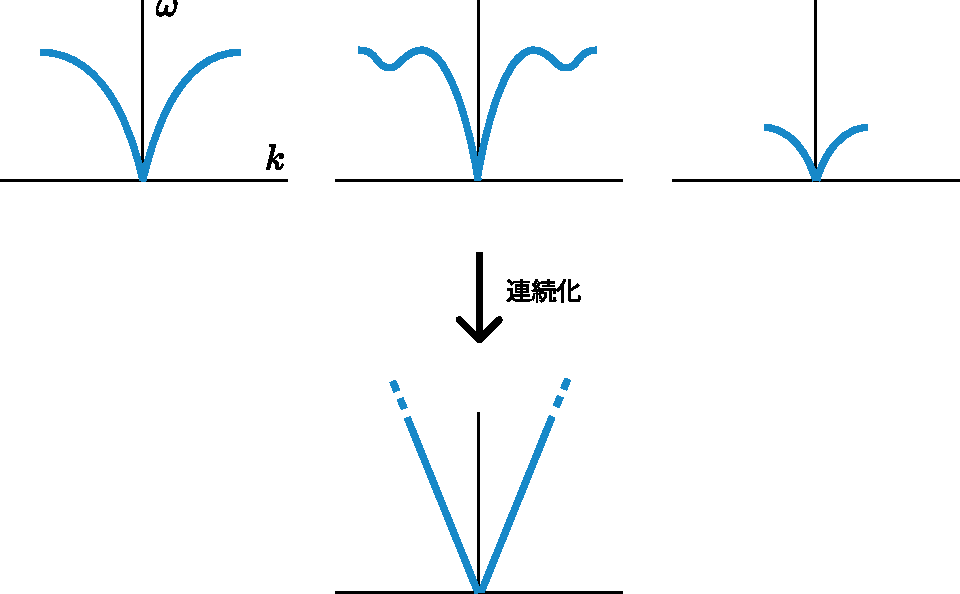
\includegraphics[width=0.5\hsize]{dispertion.pdf}
    \caption{理論の連続化の概念図}
\end{figure}
連続化した理論ともとの格子上の理論は、巨視的な物理を扱う限りは同じ結果を与える。
しかし、連続化した理論は微視的なモデルの設定の仕方によらず、普遍的である。
さらに言えば、現象論的に場の理論を扱う上で微視的なモデルについての情報は全く必要なく、空間次元や対称性といった基本的な情報といくつかの巨視的な観測量だけあれば十分である。

このことは素粒子物理学で場の量子論が非常に有効であることを説明する。
標準理論の先のミクロな物理はまだ知られていない。
超弦理論で記述される世界があるかもしれないし、時空に格子のような最小単位があるのかもしれない。
しかし幸いにも、我々の身の回りの低エネルギーな現象はミクロな物理の詳細に関係なく場の量子論で記述できる。

一方凝縮系の物理では、系の微視的な構成要素は分かっているが、それらが複雑に相互作用する結果としてマクロなスケールで非自明な現象が現れる。
このような場合にも、くりこまれた自由度に対する有効理論として場の理論は用いられる。
また臨界現象ではスケール不変な振る舞いが現れ、これは本質的に場の理論によって理解される。

\subsection{
    格子場の理論
}
% 場の理論における計算は無限の自由度を扱うせいで、しばしば発散をもたらす。
% 発散には2種類あって、
% 系の自由度の密度が無限大であることに起因する発散(紫外発散)と
% 系のサイズが無限大であることに起因する発散(赤外発散)
% がある。
% 特に紫外発散は場の理論で一般的な現象であり、無限大を避けるために正則化を行う必要がある。
% 正則化にはいくつかの方法があるが、ここでは格子による正則化を紹介する。
前の章で場の理論を統計力学系の連続極限として形式的に定義したが、この意味は真面目に考える必要がある。

まず時空上の格子点$x^μ = a n^μ,~ n ∈ ℤ^d$の全てについてデルタ関数を挿入すると、分配関数は
\begin{align}
    Z = ∫\𝒟ϕ∫∏_{n ∈ ℤ^d}\dd{ϕ_n} δ(ϕ(an)-ϕ_n)\e^{-S[ϕ]}
\end{align}
と書ける。
$\𝒟ϕ$による積分を先に行うと、
格子場の作用を
\begin{align}
    \e^{-S[a,ϕ]} = ∫\𝒟ϕ ∏_{n ∈ ℤ^d} δ(ϕ(an)-ϕ_n)\e^{-S[ϕ]}
\end{align}
と定義して、
\begin{align}
    Z = ∫∏_{n∈ℤ^d}\dd{ϕ_n}\e^{-S[a,ϕ]}
\end{align}
と書ける。
$S[a,ϕ]$は格子場の作用であり、$a$と離散的な場$ϕ_n$に依存する関数である。
このように、連続理論が定義できればそれを部分的に積分することで格子場の理論が得られる。

次に順序を逆にして、格子場の理論の$a → 0$の極限として連続理論を定義してみよう。
格子上で定義された近似的な作用$S'[a,ϕ]$を考える。
もし$a → 0$の極限で$S'[a,ϕ]$が$S[a,ϕ]$と等価ならば、
\begin{align}
    Z =\lim_{a → 0}∫∏_{n∈ℤ^d}\dd{ϕ_n}\e^{-S'[a,ϕ]}
\end{align}
と書けるだろう。
$S'[a,ϕ]$としては、Ising模型のように最近接格子間の相互作用のみを含むような単純なモデルを想定している。
一般に厳密な格子場の作用$S[a,ϕ]$はさまざまな距離の相互作用を含む。

% 簡単に分かることとして、相関距離が0でないような場の理論をつくるためには、格子場の相関距離は($a$を単位として)無限大になる必要がある。
% したがって、格子理論は$a → 0$で臨界点に漸近していく必要がある。

近似的な作用の形を決めたとしても、$a → 0$の極限をとるためには「巨視的な物理が変わらないように」作用の$a$依存性を決定しなければいけない。
% しかし、このプログラムを素朴に実行しようとすると、物理量の発散に出くわすことがある。
しかし、実は作用が場の2次形式で表されるような単純な場合(自由場の理論)を除いて、「巨視的な物理が変わらないように」とは微視的には何を意味するかが非自明な問題となる。
逆の視点から言えば、微視的なモデルが与えられていても、そこから巨視的な物理を導くのは非自明な問題である。
これらを紐解く強力な手法がくりこみ群である。

\subsection{
    くりこみ群
}
% 古典的な理論が連続理論の場合はまず正則化という処理をして、一旦離散化した理論に戻してから量子化し、それをまた連続化するという手順を行う。
% \begin{gather}
%     \t{格子理論 → 量子化 → 連続化}
%     \\
%     \t{連続理論 → 正則化 → 量子化 → 連続化}
% \end{gather}
この記事はくりこみ群の解説ではないので、詳細な計算は述べずに概念的な話に終始する。物足りない方は
\cite{altland2010condensed}の8章や
\cite{goldenfeld2018lectures}、
\cite{cardy1996scaling}
などを参照してほしい。
\begin{figure}[H]
    \centering
    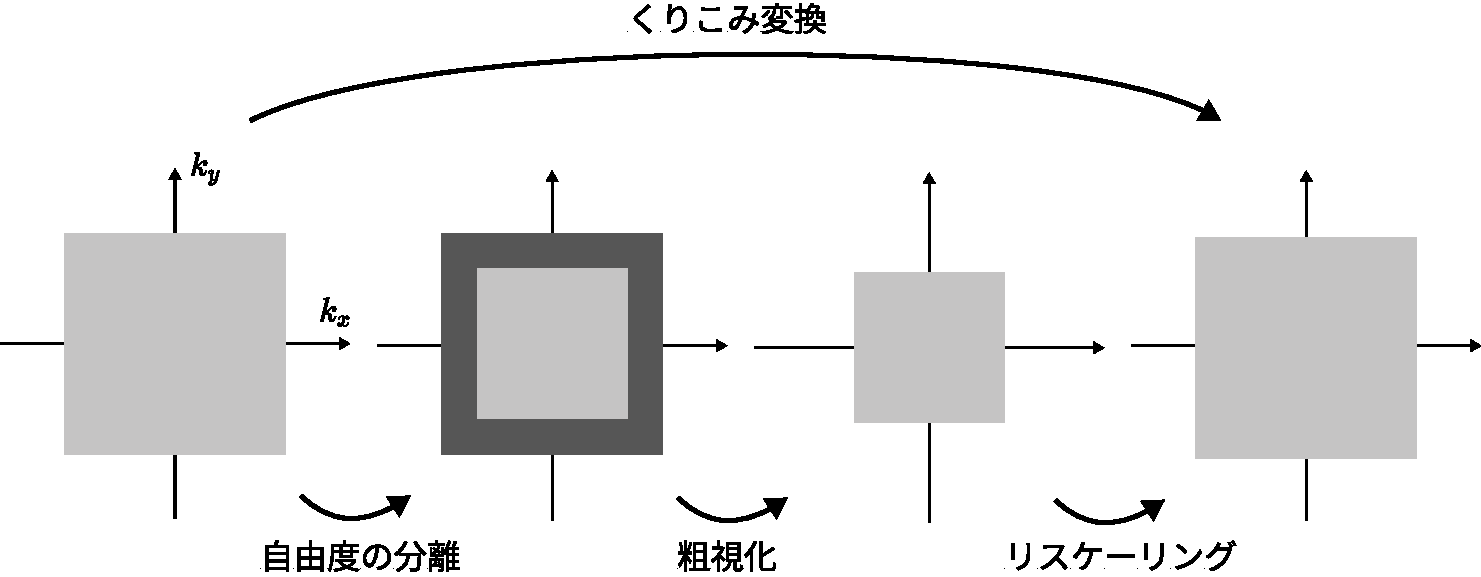
\includegraphics[width=0.7\hsize]{../images/RG.pdf}
    \caption{くりこみ変換の概念図}
\end{figure}
くりこみ群を解析計算で具体的に行う場合、運動量空間で考えることが多い。
運動量にカットオフ$Λ$をつけた系の分配関数を
\begin{align}
    Z = ∫_{|𝒌|<Λ}\𝒟ϕ\e^{-S[ϕ]}
    \label{eq: partion function before renormalization}
\end{align}
のように書く。
ただし、$∫_{|𝒌|<Λ}$は$ϕ(x)$が$|𝒌|<Λ$のFourier成分のみをもつことを表す。この式における経路積分の測度は形式的に
\begin{align}
    \𝒟ϕ = ∏_{|𝒌|<Λ}\dd{ϕ_𝒌}
\end{align}
と表される。
$|𝒌|$を通常の$L^2$ノルムではなく$L^∞$ノルム($\max|k_i|$)とすると、$|𝒌|<Λ$は立方格子のBrillouinゾーンを表し、格子場の理論が得られる。このとき$Λ$は$π/a$に対応する。
以上のような正則化
\footnote{
    いまの文脈では理論の離散化と思ってもらってもいい。
    正確には場の理論に現れる発散を抑えるための操作のことをいい、次元正則化を始め色々な方法がある。
}
は連続的な作用$S[ϕ]$が与えられれば、短波長のFourier成分を手で取り除くことで直ちに行えることに注意する。

系を粗視化したときに有効的な作用がどのように変化するかを観察するのがくりこみ群の出発点である。
実数$τ>0$に対し、場を波数が$|𝒌|<\e^{-τ}Λ$となる巨視的な成分$ϕ_\rm{s}$と$\e^{-τ}Λ<|𝒌|<Λ$となる微視的な成分$ϕ_\rm{f}$に分ける。
\footnote{sとfはslowとfastの頭文字をとった。}
またそれに対応して、作用を
\begin{align}
    S[ϕ]
    = S_\rm{s}[ϕ_\rm{s}] + S_\rm{f}[ϕ_\rm{f}] + S_\rm{c}[ϕ_\rm{s},ϕ_\rm{f}]
\end{align}
と分割する。あらわには書いていないが、これらの作用はカットオフ$Λ,\e^{-τ}Λ$に依存する。
微視的な場についての積分を先に行うと、分配関数は
\begin{align}
    Z
    &
    = ∫_{|𝒌|<\e^{-τ}Λ}\𝒟{ϕ_\rm{s}}
        \e^{-S_\rm{s}[ϕ_\rm{s}]}
    ∫_{\e^{-τ}Λ<|𝒌|<Λ}\𝒟{ϕ_\rm{f}}
        \e^{-S_\rm{c}[ϕ_\rm{s},ϕ_\rm{f}]-S_\rm{f}[ϕ_\rm{f}]}
    \∅ &
    = Z_\rm{f} ∫_{|𝒌|<\e^{-τ}Λ}\𝒟{ϕ_\rm{s}}\e^{-S_\rm{s}[ϕ_\rm{s}]}
    \⟨\e^{-S_\rm{c}[ϕ_\rm{s},ϕ_\rm{f}]}\⟩_\rm{f}
    \∅ &
    = Z_\rm{f} ∫_{|𝒌|<\e^{-τ}Λ}\𝒟{ϕ_\rm{s}}\e^{-S_\rm{eff}[ϕ_\rm{s}]}
    \label{eq: coarse graining}
\end{align}
と書ける。ここで、$S_\rm{f}$についての期待値を
\begin{align}
    \⟨A\⟩_\rm{f} ≔ \f{1}{Z_\rm{f}}∫_{\e^{-τ}Λ<|𝒌|<Λ}\𝒟{ϕ_\rm{f}}A\e^{-S_\rm{f}[ϕ_\rm{f}]},\␣
    Z_\rm{f} ≔ ∫\𝒟{ϕ_\rm{f}}\e^{-S_\rm{f}[ϕ_\rm{f}]}
\end{align}
と定義した。
また、粗視化された作用を
\begin{align}
    \e^{-S_\rm{eff}[ϕ_\rm{s}]}
    ≔ \e^{-S_\rm{s}[ϕ_\rm{s}]}\⟨\e^{S_\rm{c}[ϕ_\rm{s},ϕ_\rm{f}]}\⟩_\rm{f}
\end{align}
と定義した。この式は、微視的な自由度を積分すると、それが単に消えるのではなく、巨視的な自由度との結合を通じてくりこまれて現れてくることを意味する。

次に、粗視化の前後で作用を比較しやすくするために、
\begin{align}
    𝒌' = \e^τ 𝒌,\␣
    ϕ' = \e^{Δ_ϕτ}ϕ
\end{align}
と定義してリスケーリングを行う。
$Δ_ϕ$は$ϕ$の質量次元であり、この設定の仕方には任意性があるが、通常は運動項$∝∫\d^d{x}(∂ϕ)^2$が不変になるようにする。
素朴には$Δ_ϕ = d/2-1$だが、くりこみの効果によってここからのずれ(異常次元)が発生することがある。
リスケーリング後の(\ref{eq: coarse graining})は
\begin{align}
    Z ∝ ∫_{|𝒌'|<Λ}\𝒟{ϕ'}\e^{-S_\rm{eff}[\e^{-Δ_ϕτ}ϕ']}
    ≕ ∫_{|𝒌'|<Λ}\𝒟{ϕ'}\e^{-R_τ(S)[ϕ']}
\end{align}
と書ける。
これをもとの分配関数(\ref{eq: partion function before renormalization})と比較すると、
系の粗視化+スケール変換が作用に対する変換
\begin{align}
    S[ϕ] → R_τ(S)[ϕ]\␣ (τ > 0)
\end{align}
とみなせることが分かる。これを\textbf{くりこみ変換}と呼ぶ。
またくりこみ変換全体の集合のことを\textbf{くりこみ群}と呼ぶ。
\footnote{
    くりこみ群は正確には群ではなく半群(結合法則を満たす代数)である、と物理の文献にはよく書いてある。
    このような説明に関する注意として、まず恒等変換はくりこみ群に含めてやるのが自然なので、くりこみ群はモノイドと言うべきだと思う。
    またくりこみ群方程式を逆に解くことで、少なくとも形式的にはフローを遡ることができるので、(熱力学極限では)くりこみ変換に逆変換が存在する。
    ただしこの変換は粗視化とスケール変換によっては得られないので、くりこみ変換ではない。
}

作用を基底$O_i[ϕ]$の線型結合によって
\begin{align}
    S[ϕ] = ∑_i g_i O_i[ϕ]
\end{align}
と書くと、くりこみ変換は結合定数$g_i$についての変換となる。
$τ$が微小であるとき、$R_τ(S)[ϕ]$はもとの作用とほとんど同じであるから、$τ$についての微分方程式
\begin{align}
    \dv{g_i(τ)}{τ} = \dv{τ}R_τ(g_i) = β_i(g)
    \label{eq: flow eq}
\end{align}
を立てることができる。これを\textbf{くりこみ群方程式}と呼ぶ。
また右辺を\textbf{ベータ関数}と呼ぶ。

% 今まで抽象的な話ばかりしていたので、例としてスカラー$ϕ⁴$模型を考える。
% \begin{align}
%     S[ϕ] = ∫\d^d{x}(
%         \f{1}{2}∂_μϕ∂^μϕ+\f{g_2}{2}ϕ^2+\f{g_4}{4!}ϕ^4
%     )
% \end{align}
% これを格子正則化すると、
% \begin{align}
%     S[a,ϕ] = ∑_{n∈ℤ^d} \Q[
%         \f{1}{2}∑_{μ=1}^d\Q(\f{ϕ_{n+e_μ}-ϕ_n}{a})²
%         +\f{g_2(a)}{2}ϕ_n²+\f{g_4(a)}{4!}ϕ_n⁴
%     ]
% \end{align}
% となる。
% ここで$e_μ$は$μ$方向の単位ベクトルである。
% いま結合定数$g_2(a),g_4(a)$が$a$に依存していることに注意してほしい。
% \ref{subsec: continuum limit}で議論した弦の作用(\ref{action of string})では密度$ρ$と張力$T$は巨視的な物理量だと仮定して$a$依存性を除外していた。

% ここで$a → 0$としたときに、(格子間隔より十分大きなスケールでの)相関関数が変わらないという条件を課して、結合定数の$a$依存性を決めることにする。
% くりこみ変換の計算は具体的に摂動論を用いて実行できて、例えば$d=4$の場合に
% \begin{align}
%     (1/a)\∂{(1/a)}g_4(a) = \f{3}{16π²}g_4(a)^2 + 𝒪(g_4^3)
% \end{align}
% のような微分方程式が得られる。

\subsection{
    固定点と臨界現象
}
くりこみ群の視点から、普遍的な長距離の物理が微視的なモデルからどのように現れるかという問題を改めて考えてみよう。

まずくりこみ群の舞台として、次元や対称性のもとでありうる全ての$S[ϕ]$を集めた\textbf{理論空間}を考える。
(\ref{eq: flow eq})を解くと、理論空間内で理論が変化していく軌跡が得られる。これをくりこみ群のフローと呼ぶ。

物理的な系では、くりこみ変換を繰り返すと系に特徴的なスケールは全て積分されてしまってスケールを持たない理論に近づいていくと考えられる。
このような理論はくりこみ変換によって不変な固定点である。
すなわち、
\begin{align}
    R_τ(g_i) = g_i,\␣
    β(g_i) = 0
\end{align}
が成り立つ。
\footnote{
    Lagrangianに含まれる定数項や全微分項についての結合定数は変化しても良い。
    つまり、固定点とは理論空間全体を定数項や全微分項の分の不定性で割った同値類における固定点である。
}
後で改めて説明するが、この記事のテーマである共形場理論の正体とは、実はこの固定点である。

くりこみ変換によって相関距離は単調減少することに注目する。
相関距離とは、相関関数が
\begin{align}
    \⟨ϕ(x)ϕ(y)\⟩ ∼ \e^{-(x-y)/ξ}\␣ (|x-y| ≫ a,1/Λ)
    \label{definition of correlation length}
\end{align}
と表される時の$ξ$を指す。
\footnote{
なぜ一般に相関関数がこのような形で書けるか疑問に思うかもしれないので、簡単に導いておく。
並進対称性と回転対称性を仮定して、2つの場の座標がそれぞれ$(t,𝟎),(0,𝟎)$の場合を考える。
このとき相関関数はHamiltonianによって
\begin{align}
    \⟨ϕ(t,𝟎)ϕ(0,𝟎)\⟩ = ⟨0|\^ϕ(t,𝟎)\^ϕ(0,𝟎)|0⟩
    ≕ ⟨0|\^ϕ(0,𝟎)\e^{-\^Ht}\^ϕ(0,𝟎)|0⟩
\end{align}
と表せる。ただし、$\^H|0⟩=0$となるようにHamiltonianを定義した。
ここから相関関数は転送行列$\e^{-\^Ht}$の対角成分の1つを見ていることになる。
$t$が十分大きければ転送行列の固有値のうち主要なものからの寄与だけが残ると考えられるので、それを$1/ξ$とおくと、
\begin{align}
    \⟨ϕ(t,𝟎)ϕ(0,𝟎)\⟩ ∼ \e^{-t/ξ}
\end{align}
となり、(\ref{definition of correlation length})が得られる。
ただし、場の理論では転送行列は$∞×∞$行列であり、スペクトルは連続的なので、この議論は常に成り立つとは限らない。

座標はくりこみ変換によって$x → x' = \e^{-τ}x$と変換されるので、
$x/ξ = x'/(\e^{-τ}ξ)$となり、相関距離は$ξ → \e^{-τ}ξ$と変換される。よって単調減少する。
$ϕ$のリスケーリングは相関関数を定数倍するだけで、$ξ$には寄与しない。
}
固定点では$ξ$は変化しないので、$ξ=0$か$ξ=∞$でなければならない。
$ξ=0$の場合、各点の自由度が独立しているため、空間に依存する場を考える意味がない。
したがって、より興味深いのは$ξ=∞$の固定点である。
相関距離の発散は2次相転移の特徴だったので、この固定点は臨界点を表している。
% したがって、我々の興味を引くような場の理論は、臨界点を表す固定点に(から)無限の時間をかけて流れ込む(流れ出る)くりこみ群のフローとして表される。

固定点の近傍$g = g_0 + δg$ではベータ関数は$δg$に比例する。
すなわち
\begin{align}
    β_i(g_0+δg) ≕ -γ_{nm} δg_m
\end{align}
と書ける。
これが対角化されているとして、
\begin{align}
    γ_{ij} δg_j = y_i δg_i,\␣
    (y_i ∈ ℝ)
\end{align}
と書く。
ここで$γ_{ij}$が実数固有値を持つと仮定した。
\footnote{
    この仮定の妥当性について私はよく知らないが、多くの理論で成り立っているようである。
    複素数固有値を認めると、後で構成するスケール変換の生成子がHermite演算子になってくれないので困る。
}
$y_i$は$g_i$の質量次元を表しており、したがって$O_i[ϕ]$の質量次元は
$-y_i$である。
$O_i[ϕ] = ∫\d[d]{x}𝒪_i(x)$と表される場合、$𝒪_i(x)$の質量次元は$Δ_i = d - y_i$となる。
すると、固有ベクトルは符号によって以下の3つに分類される。
\begin{itemize}
    \item \textbf{relevant}な方向/摂動/相互作用: 
    $y_i > 0,~ Δ_i < d$
    \item \textbf{irrelevant}な方向/摂動/相互作用:
    $y_i < 0,~ Δ_i > d$
    \item \textbf{marginal}な方向/摂動/相互作用:
    $y_i = 0,~ Δ_i = d$
\end{itemize}
relevantな摂動はくりこみ変換を繰り返すことで大きくなっていき、理論はこの方向について固定点から離れていく。
irelevantな摂動はくりこみ変換を繰り返すことで小さくなっていき、理論はこの方向について固定点に近づいていく。
marginalな摂動は線形近似の範囲では一定となるが、高次の項を考えると大きくなる場合も小さくなる場合もある。

relevantな摂動を持たない固定点を\textbf{安定固定点}と呼ぶ。
またrelevantな摂動を1つでも持つ固定点を\textbf{不安定固定点}と呼ぶ。

ある点から出発してくりこみ変換を無限に繰り返していくと、やがて固定点に流れ着くと考えられる。
特定の変数が発散してしまうこともありえるが、その場合無限遠に固定点が存在すると考える。
\footnote{
    無限遠の固定点のまわりではくりこみ変換の線形化はできない。
    その場合は最も強く発散する項が不変になるように場をリスケールする。
    この代償として、運動項がくりこみ変換で変化するようになる。
    運動項が高次の微分項も含め全てゼロになる場合、空間的な相関は完全に失われる。
    このとき全ての自由度が独立に揺らいでおり、場の理論というより熱力学で記述される系となる。
}
すると、最終的にどの固定点に行き着くかによって理論空間をいくつかの領域に分割することができる。
\footnote{
    周期的な軌道に収束したり(リミットサイクル)、カオス的な挙動を示したりする可能性は考慮していない。
}
\begin{figure}[H]
    \centering
    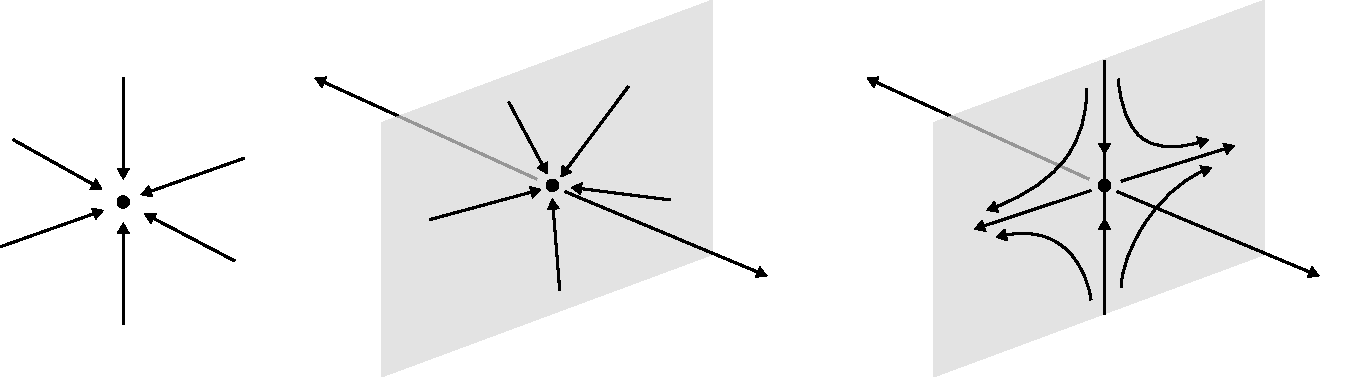
\includegraphics[width=0.8\hsize]{../images/RG_trajectory.pdf}
    \caption{relevantな方向を0個、1個、2個もつ固定点}
\end{figure}
もっともありふれたものは余次元0の多様体である。この中心にある固定点はまわりの全ての点を引き寄せ、relevantな方向をもたない安定固定点である。

次にこの領域の境界を考える。これは余次元1の多様体であり臨界面と呼ばれる。臨界面上のフローは臨界面から出ることはない。(少しでも臨界面からはみ出すと、固定点に吸い込まれてしまう。)
したがって臨界面にも固定点が現れ、それはrelevantな方向を1つもつ。

さらに、臨界面上のフローが2つの固定点に流れていくとしよう。
この間にはどちらの固定点にも流れない余次元2の臨界面が存在する。
この上にも固定点が現れ、それはrelevantな方向を2つもつ。
このように、臨界面とその上の固定点を次々に考えることができる。

ここで、1個のパラメーターをもった統計力学系を考えてみる。
これは理論空間の中で1次元の多様体をなす。
これが余次元1の臨界面と交点を持ったとしよう。
この交点は転移点となり得る。なぜならば、この点の前後で系を粗視化したときの振る舞いが不連続に変化するからである。
同様に、2個のパラメーターを調節することで起こる転移点は、余次元2の臨界面との交点に対応する。

転移点からのフローは固定点に収束する。さらに、転移点の近傍も固定点の近傍に流れていく。
微視的なモデルを多少改変したとしても、臨界面との交点は同じ固定点に流れていく。このことは臨界現象が普遍性をもつことを意味する。
同じ固定点に流れ着く転移点は同じ\textbf{普遍類(universality class)}に属するという。
代表的な例では、気液相転移の臨界点と3次元Ising模型はどちらも$ℤ_2$対称性
\footnote{
    恒等変換と符号の反転$ϕ → -ϕ$からなる群のこと。
}
をもつIsing普遍類に属することが知られている。

\subsection{
    共形場理論
}
くりこみ群の固定点は、くりこみ変換に対する不変性という意味でのスケール不変性をもつ。
しかし、ほとんどの物理的な固定点では、スケール不変性よりも強い共形不変性があることが知られている。
\footnote{
    厳密な結果では2次元三角格子上の臨界パーコレーションの共形不変性がSmirnovによって証明されている。
    詳しい話は\href{https://www.gakushuin.ac.jp/~881791/pdf/suuriPercolation.pdf}{田崎さんの解説記事}にある。
    Smirnovはさらに2次元臨界Ising模型の共形不変性を証明してFields賞を受賞している。
}
ざっくり言うと、場所ごとに倍率が異なっていてもいいスケール変換が共形変換であり、それについての不変性が共形不変性である。これについては次章で詳しく議論する。
共形不変性をもつ場の理論を\textbf{共形場理論(conformal field theory, CFT)}と呼ぶ。
臨界点にある統計力学系を無限に粗視化すると、臨界面上の固定点として共形場理論が得られる。
\begin{figure}[H]
    \centering
    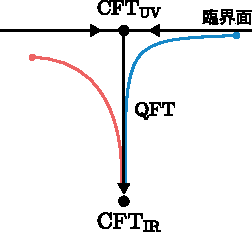
\includegraphics[width=0.4\hsize]{CFT_to_CFT.pdf}
    \caption{臨界面の近傍が粗視化によって普遍的な場の理論に漸近していく様子。}
\end{figure}
臨界点から微小にずれた系でははじめは臨界面上の固定点に近づくが、段々とrelevantな摂動の寄与が無視できなくなり、安定固定点に流される。
このときのフローは不安定固定点から出発してrelevantな方向へ流れ、安定固定点に流れ着くようなフローに漸近していく。
このフローは巨視的には格子模型と同じ物理を記述するが、いくら拡大して(=フローを遡って)も固定点から逸れていくことはなく、モデルの微細な構造は見えてこない。
これはまさに我々が場の理論に求める性質である。
したがって、(連続極限がとれる)場の理論は紫外のCFTから赤外のCFTへのくりこみ群のフローであると言える。

ここまでの議論をまとめると、共形場理論のモチベーションとして以下の2つがある。
\footnote{
    あくまで初学者の私がこれらをモチベーションに勉強したというだけである。
}
\begin{itemize}
    \item 共形場理論は臨界点にある系を無限に粗視化し、本質を取り出したモデルである。
    \item 共形場理論にrelevantな摂動を加えてくりこみ変換で下流に流してやることで、一般の場の理論が得られる。
\end{itemize}
% \printbibliography
\end{document}